% pttai: Build-Time Dataflow Validation for LLM Pipeline Graphs
% EMNLP 2026 System Demonstrations submission.
%
% Style: official ACL/EMNLP style files (acl.sty, acl_natbib.bst) fetched from
%   https://github.com/acl-org/acl-style-files (master).
% Venue is SINGLE-BLIND, so the author block is shown (no [review] anonymization).
% To produce an anonymized, line-numbered review copy instead, change the acl
% option below from `final` to `review`.
% Compile:  tectonic paper/main.tex        (or: latexmk -pdf paper/main.tex)

\documentclass[11pt]{article}

\usepackage[final]{acl}

\usepackage{times}
\usepackage{latexsym}
\usepackage[T1]{fontenc}
\usepackage[utf8]{inputenc}
\usepackage{microtype}
\usepackage{inconsolata}
\usepackage{graphicx}
\usepackage{booktabs}
\usepackage{amssymb}
\usepackage{multirow}
\usepackage{enumitem}

\newcommand{\may}{\textsc{may}}
\newcommand{\must}{\textsc{must}}
\newcommand{\code}[1]{\texttt{#1}}

\title{\code{pttai}: Build-Time Dataflow Validation for LLM Pipeline Graphs}

% TODO(author): fill in the real author block (names, affiliation, email).
\author{
  Anonymous \\
  % TODO(author): Affiliation \\
  % TODO(author): \texttt{email@domain} \\
}

\begin{document}
\maketitle

\begin{abstract}
LLM agent pipelines are graphs of model calls, tools, and branches over a shared
state. A miswired one---a node that reads a state key nothing produced, an
unwired branch, a concurrent write to a key with no reducer---does not fail when
you build it. It fails \emph{after} the model has already run, once execution
reaches the broken node, having burned tokens, latency, and (with tools) real
side effects on a run that was doomed at construction. We present \code{pttai}, a
thin declarative layer that compiles a \code{>}-wired pipeline to a native
LangGraph \code{StateGraph} and, before compiling, runs a forward
\emph{dataflow} analysis over the graph. To our knowledge this is the first
compile-time dataflow analysis for LLM agent graphs. It is a \may/\must\ fixpoint
in the tradition of definite-assignment analysis: hard errors are raised only
from the \may\ (some-path) set, so the analysis is false-positive-free by
construction---it never rejects a graph that would have run. On a
15-item bug benchmark \code{pttai} fails the build on all 15; 13 of these raw
LangGraph surfaces only at runtime or never, costing 15 wasted model calls
against \code{pttai}'s zero, with no false positives on 19 valid pipelines. The
demonstration is an interactive playground that paints the offending node red at
build time, before any model call.
\end{abstract}

\section{Introduction}

Language-model pipelines have become graphs. A retrieval-augmented QA system
retrieves passages, then answers grounded in them; an extract-then-summarize
pipeline pulls typed fields from a ticket, then writes a one-line triage summary
from those fields; a document-triage pipeline classifies an incoming message and
routes it to a specialized handler. Frameworks such as
LangGraph~\citep{langgraph} express these as explicit state-machine graphs:
nodes read and write a shared state object, edges (some conditional) move control
between them.

These graphs fail differently from ordinary programs. In a shared-state graph,
a node that reads \code{state["summary"]} before any node has written
\code{summary} does not raise when the graph is built---it raises a
\code{KeyError} at run time, once control reaches that node. By then the pipeline
has already made model calls: tokens spent, latency incurred, and, if earlier
nodes called tools, side effects committed, all on a run that was structurally
broken before it started. The same is true of an unwired conditional branch (a
routing key that resolves to nowhere) and of two parallel branches writing the
same non-reduced state key (a runtime \code{InvalidUpdateError}). We verified
that all three are recurring, publicly reported failures against raw LangGraph
(\S\ref{sec:wild}).

The root cause is that the graph builder checks \emph{structure} but not
\emph{dataflow}: LangGraph's \code{compile()} does not verify that every state
key a node reads is produced upstream. Ordinary compilers have solved the
analogous problem for decades---definite-assignment analysis rejects a Java
program that reads a local before it is assigned on some
path~\citep{jls,kildall,dragon}---but no LLM-graph framework applies it to the
graph's shared state.

We present \code{pttai}, a declarative layer over LangGraph whose contribution is
exactly this missing check.\footnote{Source, examples, benchmark, and demo:
\url{https://github.com/TeeratP/agentic-framework}.}
Our contributions are:
\begin{enumerate}[noitemsep,topsep=2pt]
  \item \textbf{A compile-time dataflow analysis for LLM agent graphs}
  (\S\ref{sec:validator}): a forward \may/\must\ fixpoint over the wired graph
  that fails the build---with zero model calls---when a node reads a key no
  upstream node produces, when a branch is unwired, or when parallel branches
  write an unreduced key. Because hard errors come only from the \may\
  (some-path) set, the analysis is \emph{false-positive-free by construction}: a
  graph that would actually run is never rejected.
  \item \textbf{An interactive demonstration} (\S\ref{sec:demo}): a playground in
  which you edit a pipeline and see the compiled LangGraph, or, when the build
  fails, the pre-compile graph with the offending node(s) painted red---the
  picture of the bug, before any model call.
  \item \textbf{An evaluation} (\S\ref{sec:eval}) on a bug benchmark
  (13 differentiating bug classes caught at build with 0 false positives on 19
  valid pipelines), a wild-bug survey grounding the taxonomy, and negligible
  build overhead with identical run-time behavior.
\end{enumerate}
\code{pttai} borrows the ``ergonomic layer over a powerful runtime'' idea from
Keras~\citep{keras}, but the ergonomics are not the contribution; the validator
is. Everything \code{pttai} builds is a plain LangGraph graph, so streaming,
async, checkpointers, and observability are inherited, not reimplemented.

\begin{figure}[t]
  \centering
  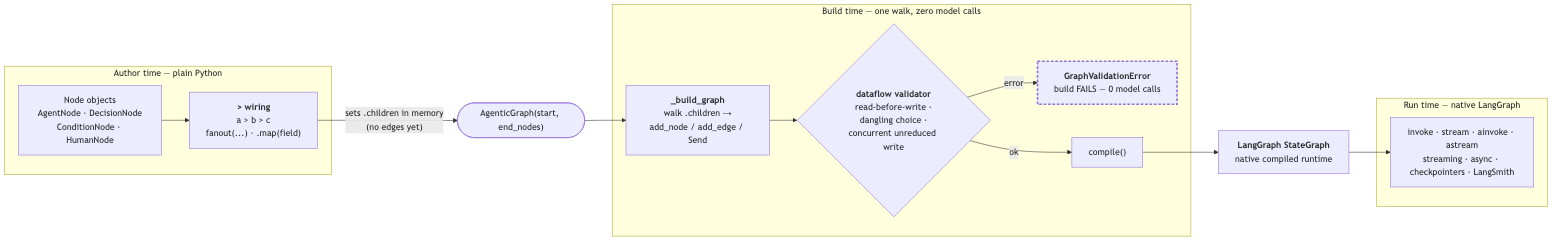
\includegraphics[width=\columnwidth]{figures/architecture.png}
  \caption{The \code{>} DSL builds a linked node structure in memory;
  \code{AgenticGraph} walks it into \code{add\_node}/\code{add\_edge}/\code{Send}
  calls; the build-time dataflow validator gates the build
  (\code{GraphValidationError} on failure, \emph{before any model call}); on
  success it compiles to a native LangGraph \code{StateGraph}.}
  \label{fig:arch}
\end{figure}

\section{System Design}
\label{sec:design}

\subsection{The \code{>} DSL and compilation}

A \code{pttai} pipeline is built by instantiating \code{Node} objects and wiring
them with \code{>} (Figure~\ref{fig:arch}). Wiring is deferred: \code{a > b} sets
\code{a.child = b} and returns \code{b}, so \code{a > b > c} builds a linked
structure in memory---no graph edges yet. \code{AgenticGraph(start, end\_nodes)}
then walks that structure and emits the actual LangGraph
\code{add\_node}/\code{add\_edge}/\code{add\_conditional\_edges} calls before
compiling. There are three node types:
\code{AgentNode} (a system-prompted model call with an internal tool-call loop),
\code{DecisionNode} (constrained structured-output routing: the model must
return one of the declared \code{choices}, wired \code{decision["c"] > handler}),
and \code{InputNode} (human-in-the-loop via LangGraph's \code{interrupt}). Fan-out
is \code{fanout(a, b)} and map-reduce is \code{.map(field)}.

Nodes read and write a shared, reducer-based state. Each node declares its
\code{reads} and \code{writes}; a node returns only the keys it updates and the
channel reducers merge them, which is what makes parallel branches and
checkpointing correct. Crucially, an \code{AgenticGraph} \emph{is} a LangGraph
\code{StateGraph} and its compiled artifact is LangGraph's
\code{CompiledStateGraph}: \code{pttai} adds a build pass on top of LangGraph and
then hands the compiled graph to it. Nothing in the runtime is reimplemented.

\subsection{The build-time dataflow validator}
\label{sec:validator}

When \code{AgenticGraph(\dots)} is constructed, it runs a static analysis over
the wired nodes and \textbf{fails the build} on a hard error, raising
\code{GraphValidationError} before \code{compile()}. This is the contribution.

\paragraph{The analysis.} During the build we record a tagged edge list:
each edge is \code{(src, dst, kind)} where \code{kind} is \code{seq} (an
unconditional, \textsc{and} edge) or \code{cond} (an exclusive, \textsc{or} edge:
a \code{DecisionNode} choice or a \code{Send} fan-out target). Over this graph we
compute, per node, two sets of available state keys by forward fixpoint:
\begin{itemize}[noitemsep,topsep=2pt]
  \item \may---keys available on \emph{some} path into the node. A
  monotone-\emph{increasing} union fixpoint.
  \item \must---keys guaranteed on \emph{every} path into the node. A
  monotone-\emph{decreasing} fixpoint.
\end{itemize}
The transfer function is the standard forward one---a node's out-set is its
in-set plus the keys it writes---with two combining rules at joins that
distinguish this from a scalar CFG analysis:
\emph{union across an \textsc{and}-parallel join} (a node after \code{fanout(a,b)}
sees both branches' writes), and \emph{intersect across an exclusive
\textsc{or}-group} (a node after a \code{DecisionNode} is guaranteed only the keys
every choice branch produces). The seed is the \emph{input} keys---reduced
channels, schema keys no node writes, and user-declared inputs---not all declared
keys; seeding with inputs rather than the whole schema is what lets the analysis
catch a read of a \emph{computed} key before its producer has run. The fixpoint
iterates until a full sweep changes nothing, bounded by the node count.

\paragraph{Soundness / no false positives.} Hard \emph{errors} are raised only
from the \may\ set: a read is an error only when the key is available on
\emph{no} path into the node. If a key is available on some but not all paths
(\may\ but not \must), that is a \emph{warning}, never a build failure. So the
validator never rejects a graph that would actually run---false-positive-freedom
is a property of raising errors from the some-path set, exactly as
definite-assignment analysis reports ``used before assigned'' only when
\emph{no} path assigns the variable~\citep{jls,nielson}. The \must\ set only
drives warnings.

\paragraph{What it checks.} On top of the dataflow sets, \code{pttai} raises
seven error classes and four warning classes (Table~\ref{tab:checks}). Errors
fail the build; warnings surface in a \code{model.summary()}-style table and can
be promoted to errors with \code{strict=True}.

\begin{table}[t]
  \centering
  \small
  \begin{tabular}{@{}p{0.42\columnwidth}p{0.5\columnwidth}@{}}
    \toprule
    \textbf{Error (fails build)} & \textbf{Condition} \\
    \midrule
    read-before-write & reads a computed key produced only downstream / on a
    sibling branch (\may) \\
    undeclared key & reads/writes a key absent from the state schema \\
    concurrent write, no reducer & two parallel branches write the same
    non-reduced key \\
    dangling choice & a \code{DecisionNode} choice with no wired handler \\
    dead-end node & a non-terminal node with no child \\
    duplicate node name & two distinct nodes share a name$^\dagger$ \\
    prompt/read mismatch & a \code{node\_prompt} \code{\{placeholder\}} that is
    not a declared scalar read \\
    \midrule
    \textbf{Warning (build succeeds)} & \textbf{Condition} \\
    \midrule
    some-paths read & key in \may\ but not \must \\
    optional read unmet & \code{reads=["x?"]} never produced \\
    unreachable node & not reachable from the start node \\
    end node w/ children & a declared end node still has a child \\
    \bottomrule
  \end{tabular}
  \caption{The validator's error and warning classes. $^\dagger$Duplicate names
  and dead ends are raised structurally during the build walk (as
  \code{ValueError}); the rest come from the dataflow pass. A dead read (a scalar
  read never interpolated) is an additional warning.}
  \label{tab:checks}
\end{table}

\section{Demonstration}
\label{sec:demo}

The demonstration is a browser playground (Figure~\ref{fig:demo}). A reviewer
edits a small \code{pttai} snippet---one of the shipped NLP pipelines (RAG QA,
extract$\rightarrow$summarize, document triage) or their own---and submits it. On
a clean build the playground renders the \emph{compiled LangGraph} as a
node/edge diagram plus the validator's \code{summary()} table (every node's
reads, writes, and available keys). The intended live moment: take a working
RAG-QA pipeline and reorder two nodes so the answer step reads \code{passages}
before the retriever runs. Raw LangGraph would compile this and only fail after
the retrieval model call. \code{pttai} instead rejects it at build: the diagram
is redrawn from the pre-compile wiring with the \textbf{offending node painted
red} and the exact error attached (``\code{reads computed key 'passages' but no
upstream node produces it}''), with \emph{zero model calls made}. The reviewer
sees the picture of the bug before running anything.

Because the playground \code{exec}s user-supplied code, it is sandboxed for
public hosting: the snippet is size-capped, AST-checked (imports allow-listed to
\code{pttai}/\code{typing}/safe stdlib; dunder access and dangerous builtins such
as \code{eval}/\code{open}/\code{\_\_import\_\_} rejected), run with a restricted
\code{\_\_builtins\_\_}, and executed under a per-request timeout. The model
backend is an offline fake, so the demo needs no API key and makes no network
call. A \textless2.5-minute screencast accompanies the submission.

\begin{figure}[t]
  \centering
  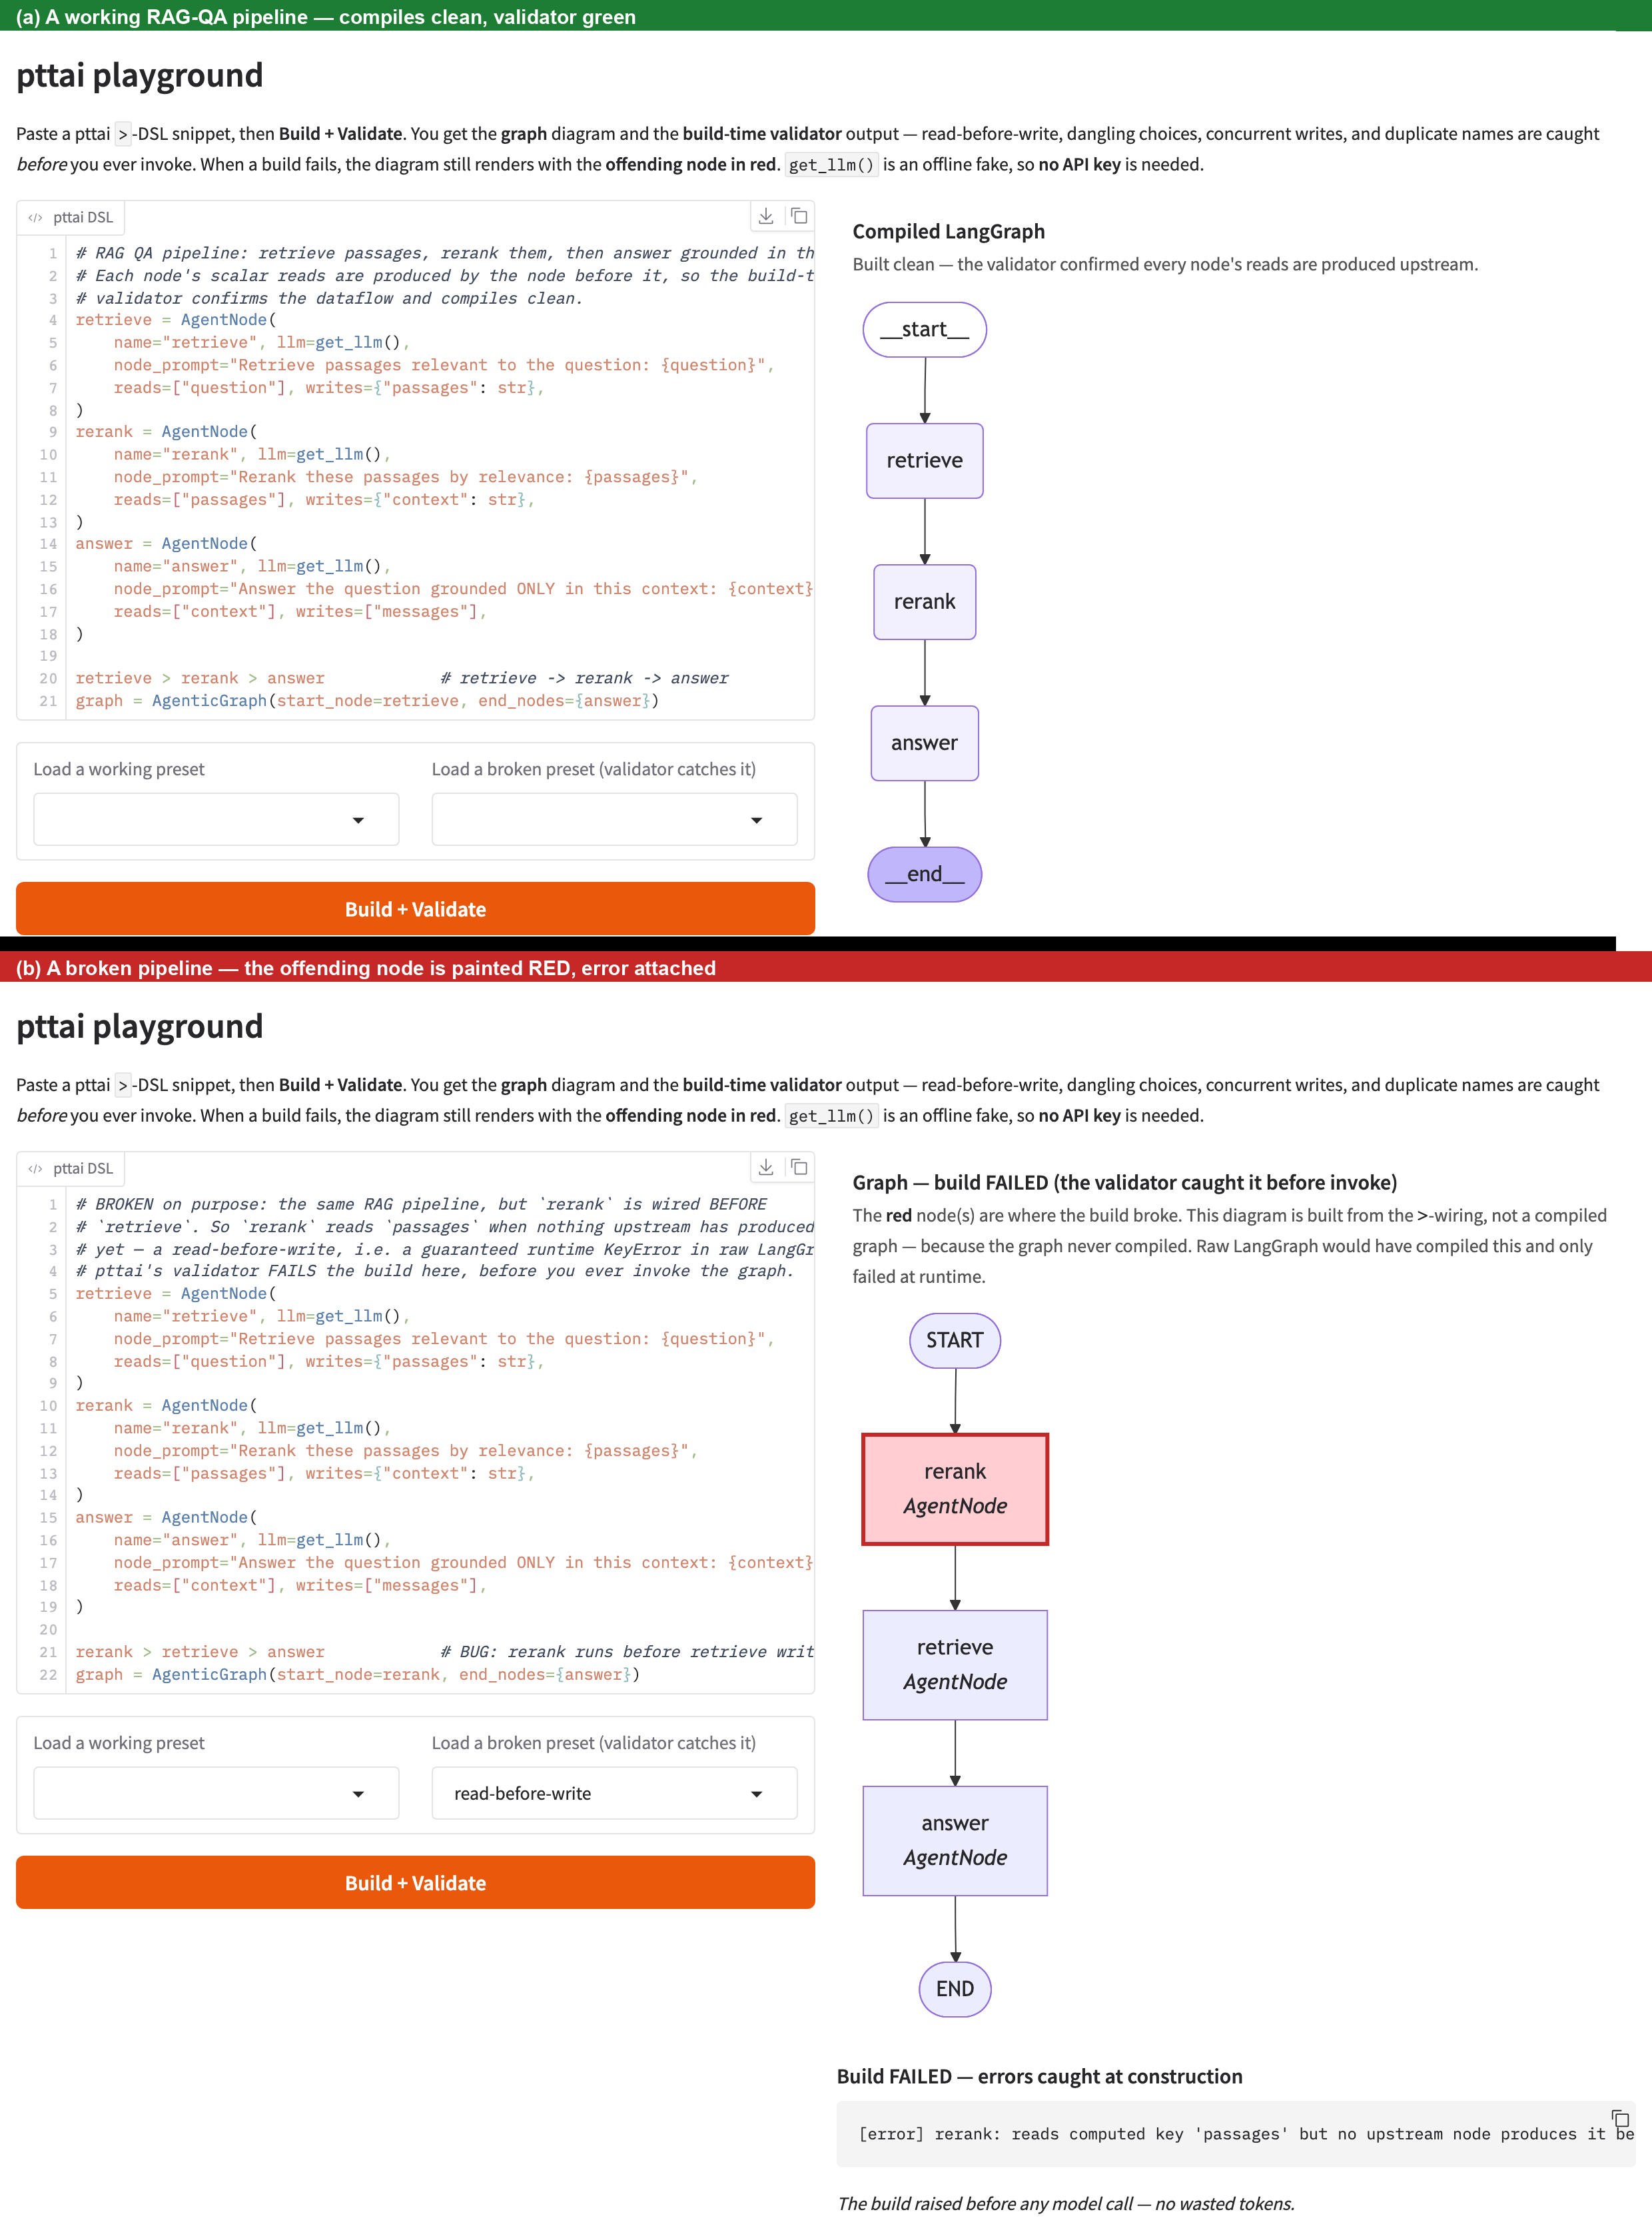
\includegraphics[width=\columnwidth]{figures/demo_screenshot.png}
  \caption{The playground. A broken pipeline is rejected at build time and drawn
  with the offending node in red and the validator error attached---no model
  call is made.}
  \label{fig:demo}
\end{figure}

\section{Evaluation}
\label{sec:eval}

All evaluations run offline (no API key); the harness is in the repository under
\code{eval/}.

\paragraph{Bug benchmark.} We built \code{bugbench}, 15 buggy pipelines (three
each of read-before-write, dangling choice, dead-end; two each of concurrent
unreduced write, prompt/read mismatch; two duplicate-name) and 19 valid
pipelines (the shipped example suite). For each we record whether \code{pttai}
fails the build and how many model calls each framework wastes before the bug
surfaces. \code{pttai} fails the build on \textbf{all 15} buggy pipelines with
the correct diagnostic, at a median of under 1\,ms and \textbf{0} wasted model
calls. Raw LangGraph catches only the 2 duplicate-name cases at build; the other
\textbf{13} it surfaces at run time (10 as \code{KeyError} /
\code{InvalidUpdateError} after the model has run) or never (3 dead-end cases
loop silently). Across the buggy set, LangGraph wastes \textbf{15} model calls to
\code{pttai}'s \textbf{0}. On the 19 valid pipelines \code{pttai} raises
\textbf{0 false positives} (0 spurious build failures)---consistent with the
some-path error rule. So on the differentiating classes the catch rate is
13/13 with 0 false positives; duplicate names are caught by both frameworks and
are not a differentiator.

\paragraph{Externally-grounded study (in progress).} A benchmark authored by us
invites the objection that the validator catches only the bugs its author
planted. We therefore designed a complementary study
(\code{eval/llmgen/}) in which a frontier model generates pipelines from short
NLP task specs---given the docs and \emph{never told to write bugs}---and every
generated pipeline is built and adjudicated, so the bug distribution comes from
real AI-written agent code rather than a hand-picked corpus. The scoring path is
proven offline on a committed sample set of 9 pipelines (4 clean, 5 buggy): 5
flagged, \textbf{0 false positives}, of which raw LangGraph would surface 4 only
at run time and 1 silently. \textbf{The headline numbers require an API key and a
generation run that the build environment cannot perform; they are reported as a
placeholder and must be filled from a keyed run before submission.}
% TODO(author): run eval/llmgen/run_study.sh with an API key, adjudicate, and
% fill the headline N / flag-rate / adjudicated-FP-rate here from results.json.

\paragraph{Wild-bug survey.}
\label{sec:wild}
To show the taxonomy is not author-imagined, we mined public issue trackers for
each targeted class (Table~\ref{tab:wild}): nine independent, verified reports
against raw LangGraph, at least two per class. Every one is a runtime failure or
a non-terminating graph that \code{pttai}'s build-time check would have caught
first. (Duplicate names and the prompt/read check are excluded here: the former
both frameworks already catch at build, and the latter is a
\code{pttai}-internal reformulation of a generic \code{str.format} error with no
LangGraph-specific report.)

\begin{table}[t]
  \centering
  \small
  \begin{tabular}{@{}p{0.6\columnwidth}c@{}}
    \toprule
    \textbf{Bug class (runtime symptom)} & \textbf{Reports} \\
    \midrule
    read-before-write (\code{KeyError} on a state key) & 2 \\
    concurrent write, no reducer (\code{InvalidUpdateError}) & 3 \\
    dangling conditional edge & 2 \\
    dead-end / non-terminating graph & 2 \\
    \midrule
    \textbf{Total} & \textbf{9} \\
    \bottomrule
  \end{tabular}
  \caption{Independent, publicly reported wild bugs against raw LangGraph, by
  targeted class (details and issue links in the repository's
  \code{docs/EVIDENCE.md}).}
  \label{tab:wild}
\end{table}

\paragraph{Conciseness (a side effect).} Across 12 canonical pipelines (the
agentic-pattern and basics suites) ported both ways, the \code{pttai} versions
total 113 lines against 281 for hand-written LangGraph---about 60\% fewer
(Figure~\ref{fig:loc}). This is a consequence of folding \code{add\_node} /
\code{add\_edge} / structured-output routing / the tool-call loop into the node
abstractions, not the point of the system; the validator is.

\begin{figure}[t]
  \centering
  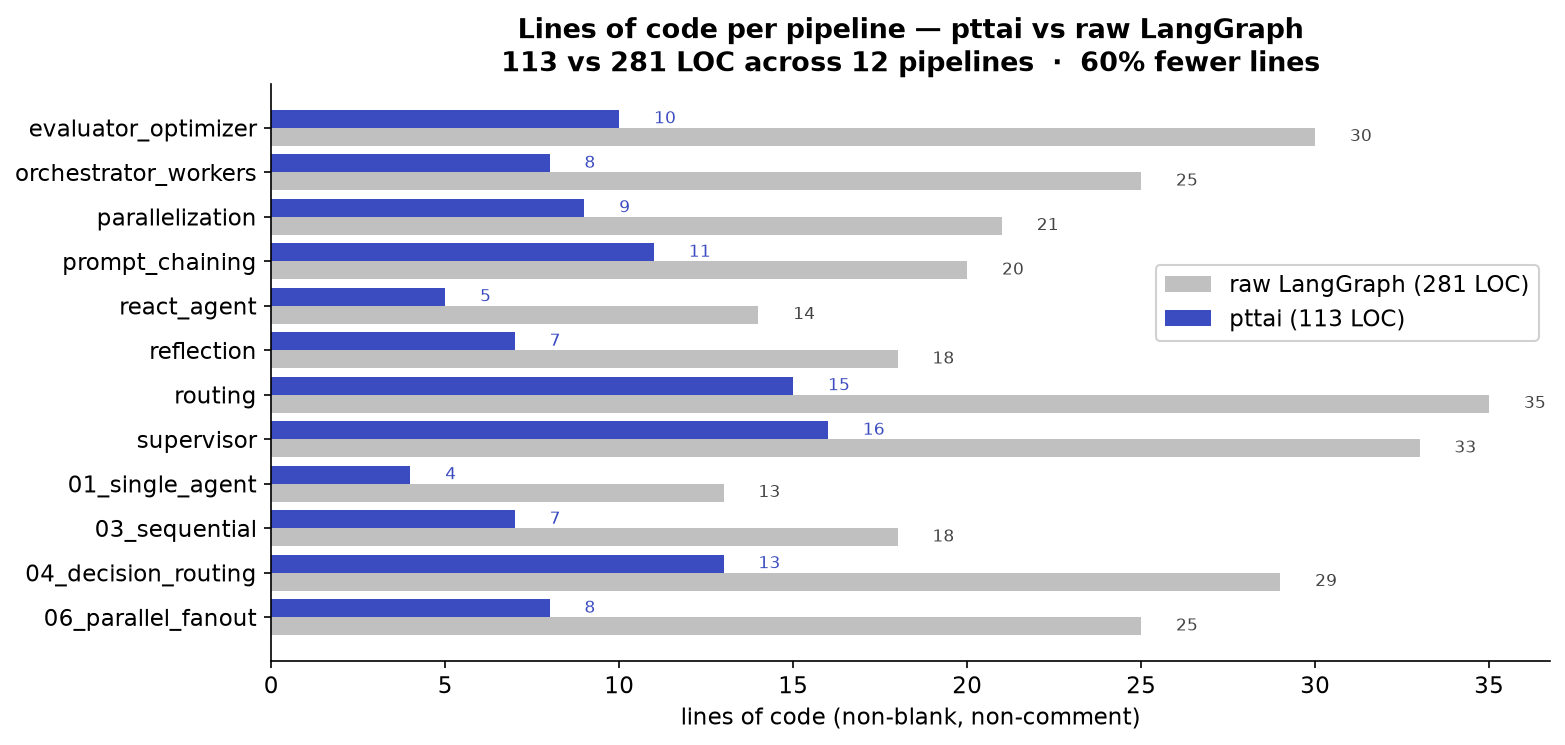
\includegraphics[width=\columnwidth]{figures/loc_comparison.png}
  \caption{Lines of code, \code{pttai} vs.\ hand-written LangGraph, across 12
  canonical pipelines (113 vs.\ 281 lines total).}
  \label{fig:loc}
\end{figure}

\paragraph{Overhead.} The added build pass (wiring + full dataflow validation +
compile) has a sub-millisecond median and is within measurement noise of a bare
LangGraph \code{compile()}; because \code{pttai} compiles to a native
\code{CompiledStateGraph}, run time is LangGraph---identical model-call count and
identical output.

\section{Related Work}
\label{sec:related}

\code{pttai} is complementary to, not a replacement for, existing frameworks; it
adds a static dataflow check none of them performs and compiles down to
LangGraph. \textbf{LangGraph}~\citep{langgraph} is the runtime \code{pttai}
targets; its \code{compile()} runs basic structural checks (it raises on a node
with no path to the end) but does not analyze which state keys are produced
before they are read---the gap this work fills. \textbf{DSPy}~\citep{dspy}
optimizes prompts and demonstrations against a metric; its control flow is
arbitrary Python, so there is no declared graph to check statically.
\textbf{LMQL}~\citep{lmql} and \textbf{Guidance}~\citep{guidance} constrain
\emph{within} a single generation (decoding, output structure) rather than across
a multi-node graph. \textbf{CrewAI}~\citep{crewai} orchestrates via roles and a
sequential/hierarchical process, with no declared node/edge graph or dataflow
validation. \textbf{AutoGen}'s GraphFlow~\citep{autogen} and
\textbf{LlamaIndex} Workflows~\citep{llamaindex} do validate graph
\emph{structure} (entry points, reachability, event-type wiring) before running,
and \textbf{Haystack}~\citep{haystack} type-checks explicit component
connections---but none performs a shared-state \emph{dataflow} analysis
(read-before-write / concurrent-unreduced-write), and thus none has a
false-positive guarantee to offer. To our knowledge \code{pttai} is the only one
of these that runs a build-time state-key dataflow analysis, and the only one
that lowers to an established graph runtime rather than shipping its own.

\section*{Limitations}

The dataflow analysis reasons about state-key \emph{availability}, not
\emph{types or values}: it verifies that a key a node reads is produced upstream,
not that its value has the expected type or is non-empty. A key produced with the
wrong type still passes. The \must\ (all-paths) set over-approximates
exclusivity in one case---a decision handler that merges back via an
unconditional edge unions into the successor's \must\ set as if unconditional---
which can only \emph{under}-warn (miss a some-paths warning); it never produces a
wrong hard error, since errors come from \may\ only. The analysis is intentionally
sound-for-errors rather than complete: it will not flag a semantic bug that is
nonetheless well-formed dataflow (e.g., a prompt that asks for the wrong thing).
The wild-bug survey is a targeted sample of public reports, not an exhaustive
census, and establishes that the classes occur, not their frequency. Finally,
the externally-grounded LLM-generation study is designed and its scoring path
verified, but its headline numbers await a keyed generation run
(\S\ref{sec:eval}); we do not report them here and do not claim them.

\section*{Ethics and Broader Impact}

\code{pttai}'s goal is to catch broken agent pipelines \emph{before} they run,
which directly reduces wasted model calls---and thus the tokens, cost, latency,
and energy spent on runs that were doomed at build time---and avoids committing
tool side effects on such runs. The public playground \code{exec}s
user-submitted code; we sandbox it (allow-listed imports, restricted builtins,
AST rejection of dangerous calls, size and time caps, offline fake model) so that
hosting it does not expose the host, but we note that \code{exec}-based sandboxes
are best-effort and a hardened deployment should add OS-level isolation. The
validator makes no claim about the \emph{safety, factuality, or bias of model
outputs}; it checks pipeline dataflow, not what the models say. \code{pttai} is
released under the MIT license.

\bibliography{refs}

\appendix

\section{Reproducing the evaluation}
\label{app:repro}

All numbers are produced offline (no API key) from the repository:
\code{eval/bugbench/run.py} regenerates \code{eval/bugbench/results.csv} (the 15
buggy / 19 valid outcomes and per-pipeline wasted-call counts);
\code{eval/loc\_compare.py} regenerates \code{eval/loc\_results.csv} (the 113
vs.\ 281 line counts over 12 pipelines); \code{eval/overhead.py} prints the
build-time and runtime-parity measurements; and
\code{eval/llmgen/score.py --gen-dir samples} runs the sample-set self-test of
the externally-grounded study. The wild-bug reports with issue links are in
\code{docs/EVIDENCE.md}.

\section{Example: a validated NLP pipeline}
\label{app:example}

The extract-then-summarize pipeline. The \code{extract} node returns typed
structured output; the \code{summarize} node reads those scalar fields and the
validator confirms, at build time, that each is produced upstream before it is
read.

\begin{quote}\small\ttfamily
extract = AgentNode(llm=llm,\\
\ \ node\_prompt="Extract fields: \{ticket\}",\\
\ \ reads=["ticket"],\\
\ \ writes=\{"product": str, "severity": int\})\\
summarize = AgentNode(llm=llm,\\
\ \ node\_prompt="severity-\{severity\} on \{product\}",\\
\ \ reads=["product", "severity"],\\
\ \ writes=["summary"], output\_field="summary")\\
extract > summarize\\
AgenticGraph(start\_node=extract,\\
\ \ end\_nodes=\{summarize\})
\end{quote}

Swapping the two nodes (\code{summarize > extract}) makes \code{summarize} read
\code{product} and \code{severity} before \code{extract} produces them; the build
fails with a read-before-write error and no model call is made.

\end{document}
